\documentclass[8pt,pdf,hyperref={unicode}]{beamer}

\mode<presentation>
{
\usetheme{boxes}
\beamertemplatenavigationsymbolsempty

\setbeamertemplate{footline}[page number]
\setbeamersize{text margin left=0.5em, text margin right=0.5em}
}

\usepackage[utf8]{inputenc}
\usepackage[english, russian]{babel}
\usepackage{bm}
\usepackage{multirow}
\usepackage{ragged2e}
\usepackage{indentfirst}
\usepackage{multicol}
\usepackage{subfig}
\usepackage{amsmath,amssymb}
\usepackage{enumerate}
\usepackage{mathtools}
\usepackage{comment}
\usepackage{multicol}
\usepackage{svg} 

% [inkscapeformat=png]

\usepackage[all]{xy}

\graphicspath{ {./images/} }

\usepackage{tikz}
\usetikzlibrary{positioning,arrows}

\tikzstyle{name} = [parameters]
\definecolor{name}{rgb}{0.5,0.5,0.5}

\usepackage{caption}
\captionsetup{skip=0pt,belowskip=0pt}

\newtheorem{rustheorem}{Теорема}
\newtheorem{russtatement}{Утверждение}
\newtheorem{rusdefinition}{Определение}

% colors
\definecolor{darkgreen}{rgb}{0.0, 0.2, 0.13}
\definecolor{darkcyan}{rgb}{0.0, 0.55, 0.55}

\AtBeginEnvironment{figure}{\setcounter{subfigure}{0}}

\captionsetup[subfloat]{labelformat=empty}

%----------------------------------------------------------------------------------------------------------

\title[One slide m1p]{One slide m1p}
\author{Melikhov Dmitry}

\institute[]{MSU}
\date[2022]{\today}

%---------------------------------------------------------------------------------------------------------
\begin{document}

%\begin{frame}
%\titlepage
%\end{frame}


%----------------------------------------------------------------------------------------------------------
\section{About task}
\begin{frame}{Детекция галлюцинаций больших языковых моделей}
\begin{columns}
% Column 1   
\begin{column}{0.4\textwidth}
    Задача: выделить фрагменты-галлюцинации -  классификация токенов (sequence labeling).
    $x_i \rightarrow y_i = \{0, 1\}$. Если $y_{i} = 1$, то $i$-й токен считается галлюцинацией.\\
    Эксперимент 1: instruction-based подход. Использована генеративная модель \texttt{Meta-Llama-3-8B} с промптом - детектировать галлюцинации.
    Выборка из 50 размеченных QA сообщений на английском.\\
    Результаты: распределение IoU на 50 объектах - рис. \ref{hist}
    Средний IoU: \textbf{0.3975}\\
    Будущий эксперимент 2: Анализ временного ряда логитов токенов.\\
    Будущий эксперимент 3: дообучение Token classification модели минимизацией бинарной кросс-энтропии:
    $$
    \mathcal{L}(y, \hat{y}) = \sum_{i} logloss(y_{i}, \hat{y}_{i}) \rightarrow \min
    $$
    $$
    logloss(y, \hat{y}) = - y log(\hat{y}) - (1 - y) log(1 - \hat{y})
    $$
\end{column}
% Column 2
\begin{column}{0.6\textwidth}
    \begin{figure}
        \centering
        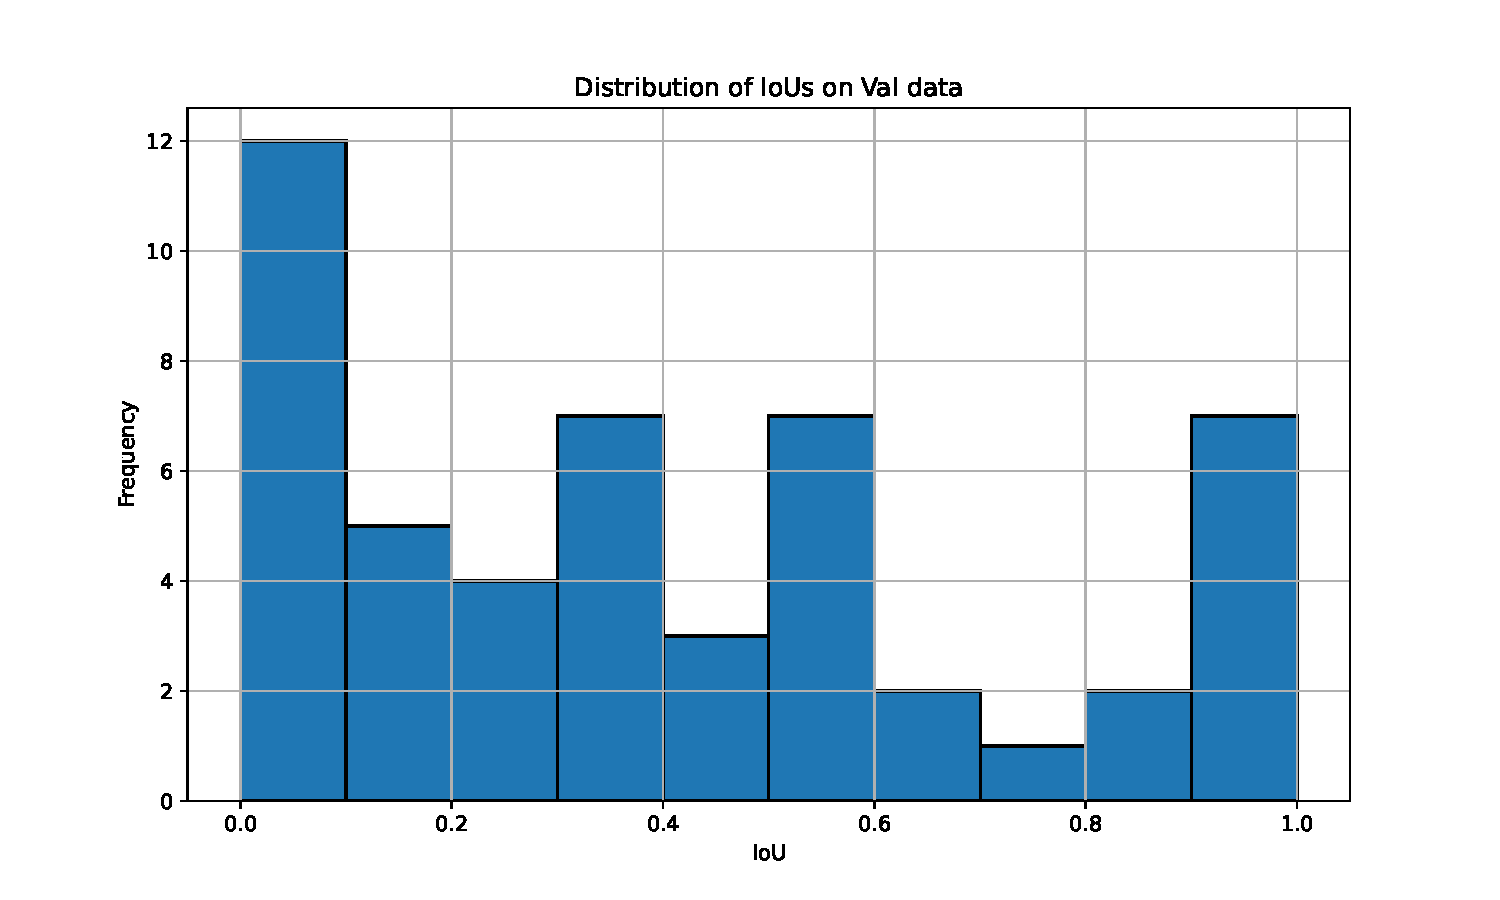
\includegraphics[width=0.8\linewidth]{images/ious_histogram.pdf}
        \label{hist}
        \caption{Результаты эксперимента 1}
    \end{figure}
    \begin{figure}
        \centering
        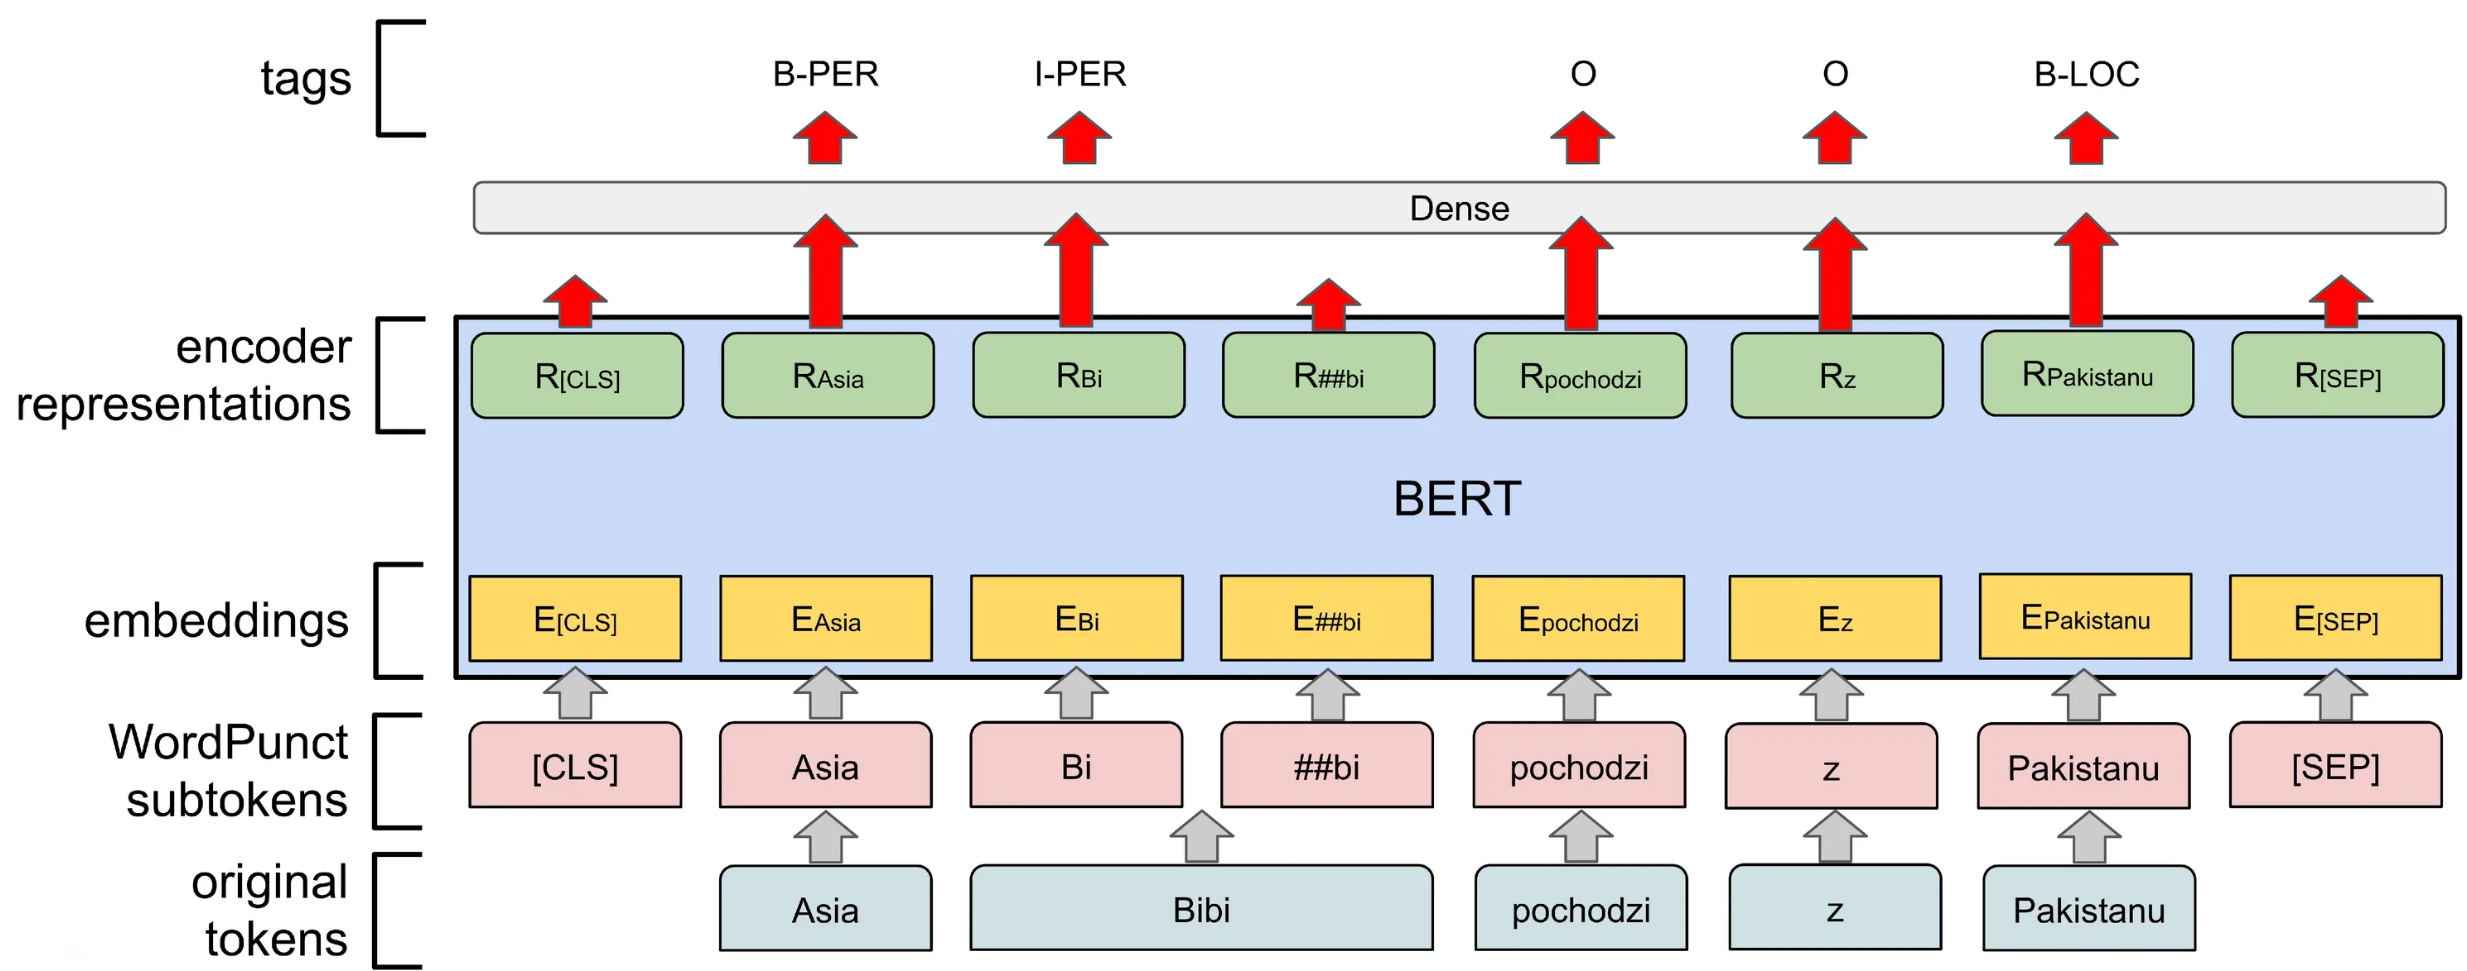
\includegraphics[width=1\linewidth]{images/bert_architecture.png}
        \label{hist}
        \caption{Планы на эксперимент 2. Архитектура BERT NER}
    \end{figure}
\end{column}
\end{columns}


\end{frame}
\end{document} 